\chapter{Objekt-Semantik}

\subsubsection*{Klassendiagramm (Struktur)}
... beschreibt den Aufbau und das Zusammenspiel von Klassen innerhalb des Systems. Meist auf Basis von Dingen.

\begin{figure}[hbt]
  \centering
  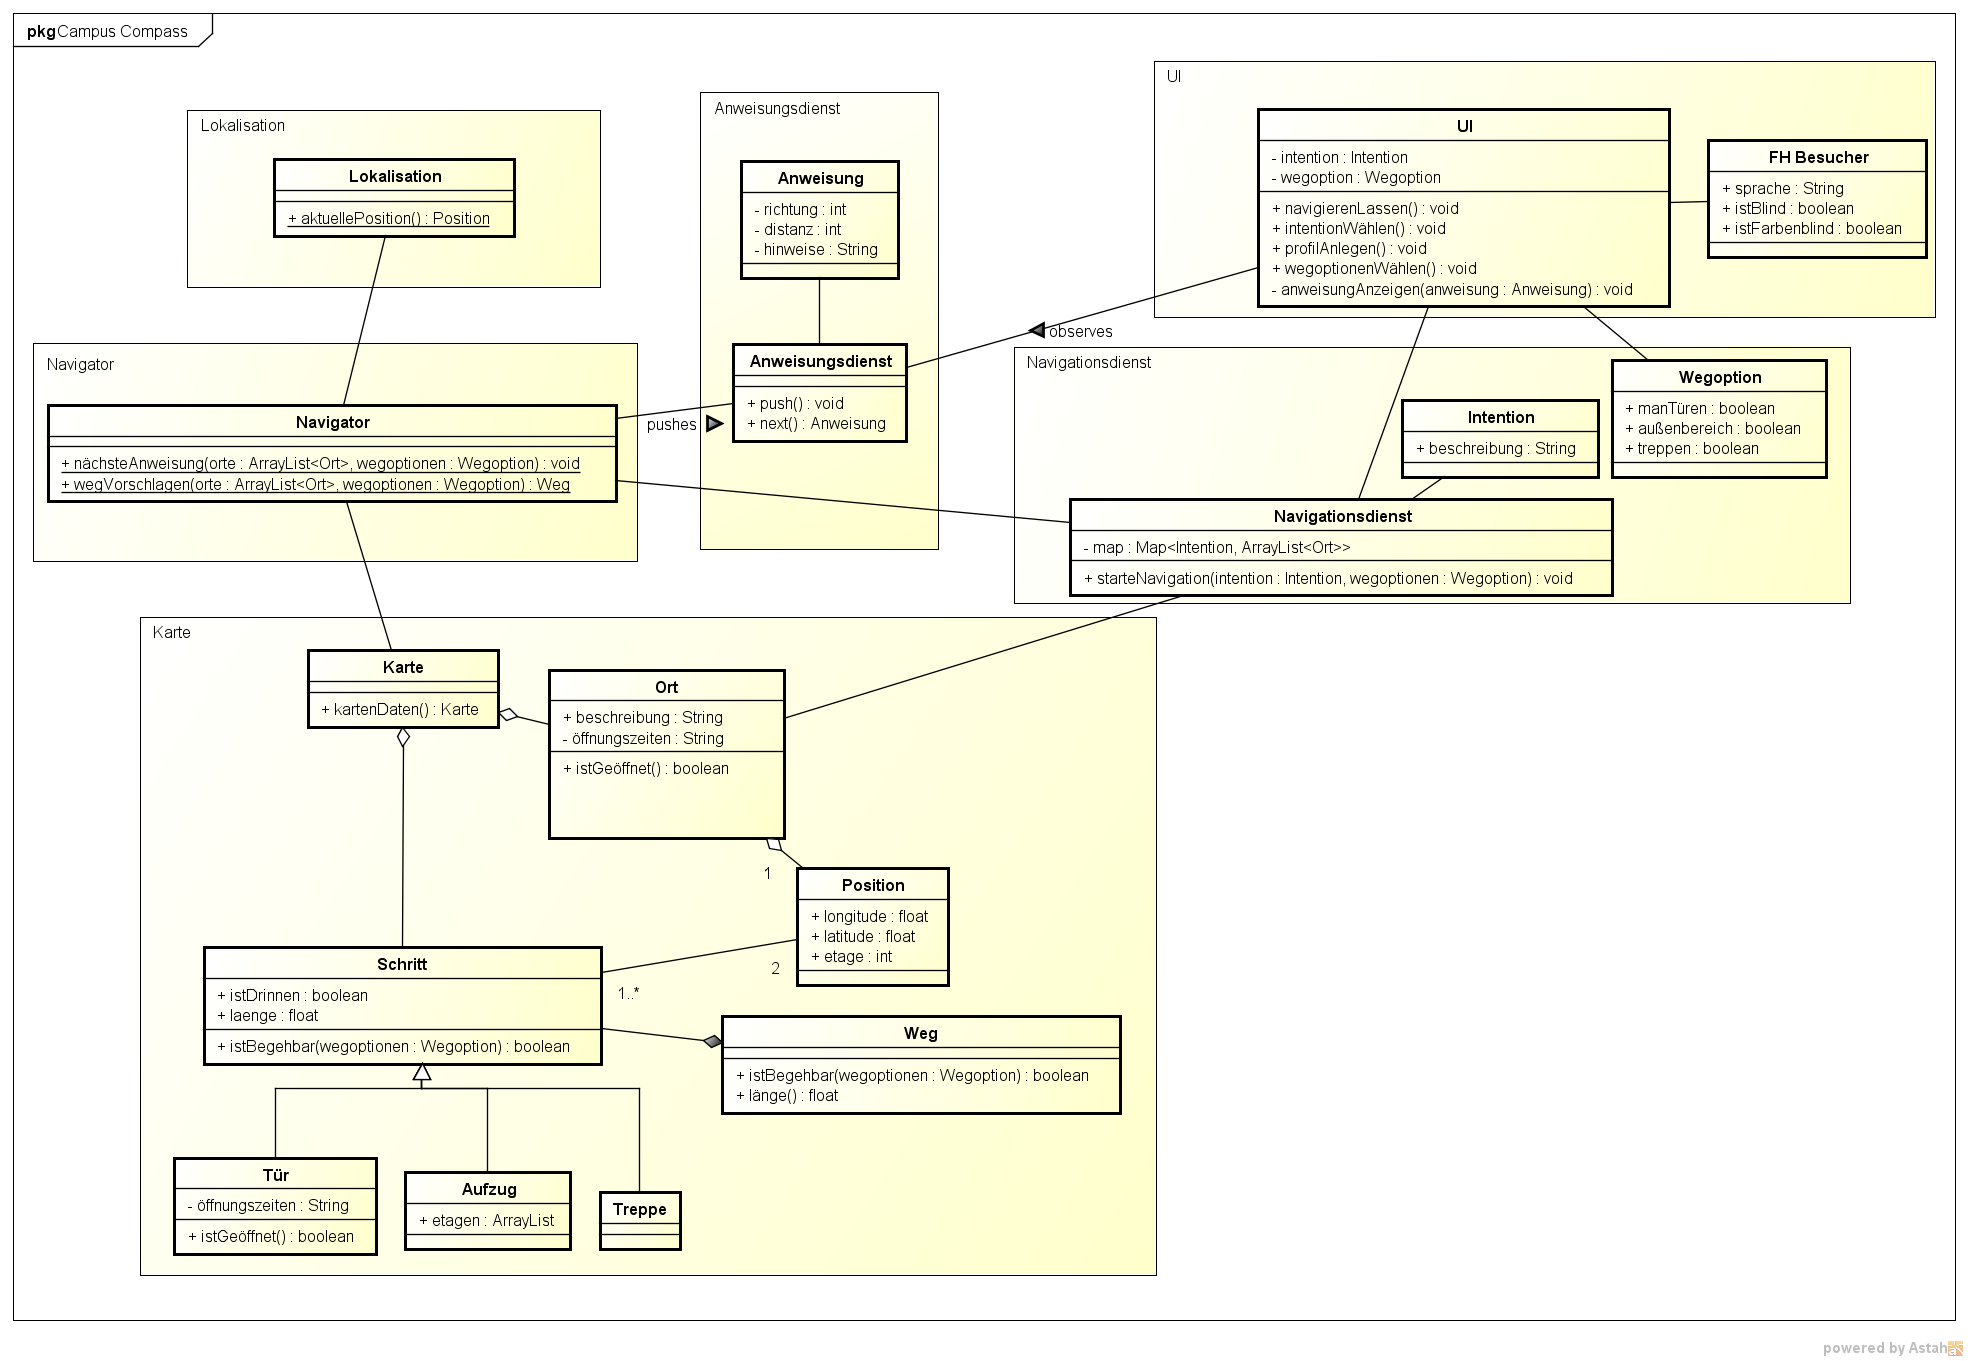
\includegraphics[width=\linewidth]{img/klassendiagramm.png}
  \label{img:klassendiagramm}
  \caption{Klassendiagramm}
\end{figure}

Im Klassendiagramm zu sehen, sind die einzelnen Klassen des Systems, gekapselt in Komponenten. Die einzelnen Komponenten, welche aus einer oder mehrerer Klassen bestehen, finden sich später im Komponentendiagramm wieder. Durch die Attribute ohne Methoden der Klassen wird ihr Zweck verdeutlicht.

\subsubsection*{Zustandsdiagramm (Verhalten)}
... zeigt den Zustand eines Obejkts zur Laufzeit.

\begin{figure}[hbt]
  \centering
  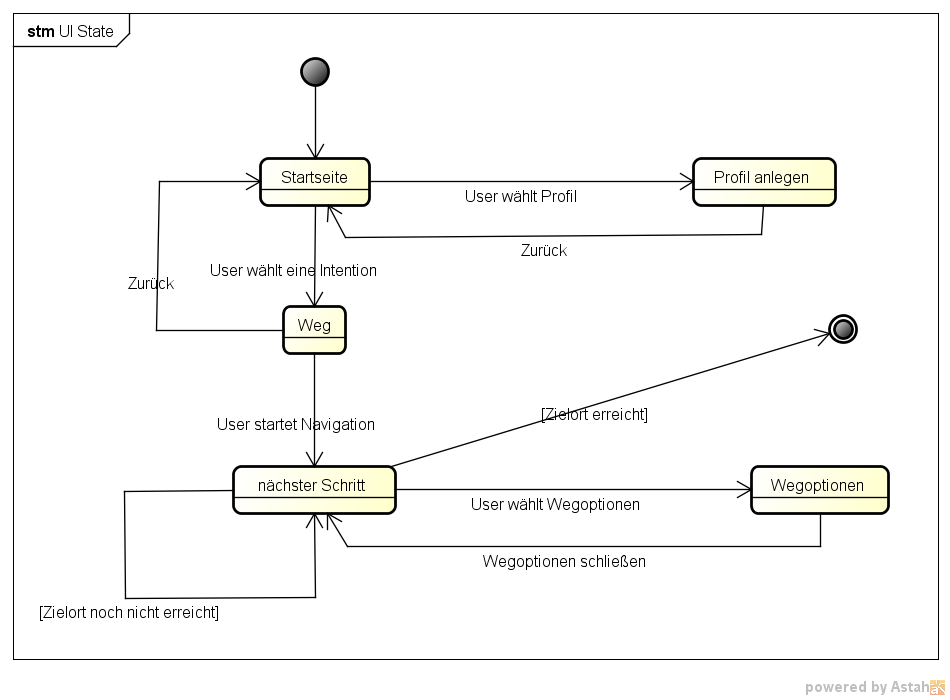
\includegraphics[width=\linewidth]{img/zustandsdiagramm.png}
  \label{img:zustandsdiagramm}
  \caption{Zustandsdiagramm}
\end{figure}

Im gezeigten Zustandsdiagramm sind die möglichen Veränderungen/Zustände des User Interface zu erkennen. Es beschreibt somit die mögliche Navigation des Systems durch das User Interface der App. Man erkennt ebenfalls, dass einige Zustände zu den zuvor gezeigten Use Cases passen.

\newpage

\subsubsection*{Sequenzdiagramm (Verhalten)}
... beschreibt die Interaktion (Kommunikation) von Objekten/Komponenten im zeitlichen Verlauf in einer bestimmten Szene.

\begin{figure}[hbt]
  \centering
  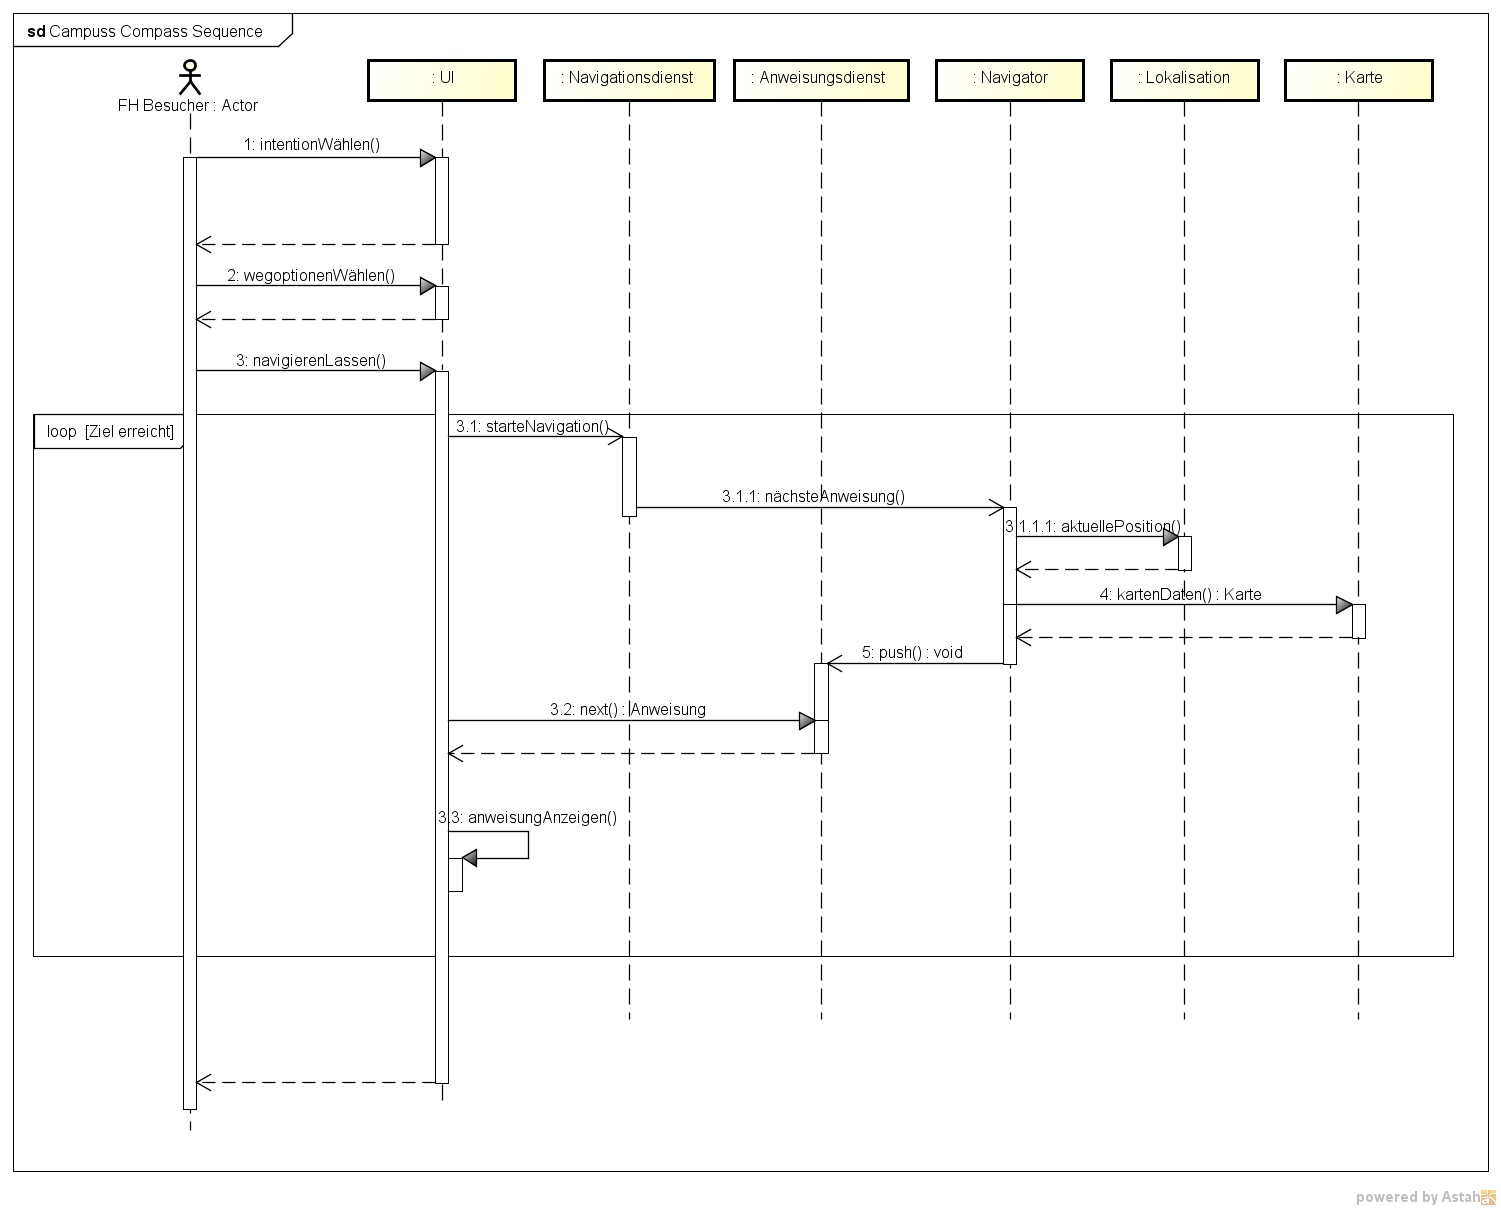
\includegraphics[width=\linewidth]{img/sequenzdiagramm.png}
  \label{img:sequenzdiagramm}
  \caption{Sequenzdiagramm}
\end{figure}

\noindent Im Sequenzdiagramm schön zu erkennen, ist die Kommunikation zwischen \gls{fhbesucher} und der Komponente UI. Diese Kommunikation macht deutlich, dass der \gls{fhbesucher} nicht an der internen Kommunikation der App beteiligt ist. Ist die \gls{navigation} gestartet, beginnt innerhalb des Loops ein Folge von internen Methodenaufrufen. Der Loop endet mit dem Anzeigen der letzten Anweisung an den \gls{fhbesucher} bevor dieser das Ziel erreicht.